\subsubsection{Theoretical Student-Teacher Average Generalization Error \texorpdfstring{$(\AVGSTGE)$}{(AVGSTGE)}}
\label{sxn:SMOG_main-st_av}

Here, we seek a simple, formal expression for the
\StudentTeacher Average \GeneralizationError, $\AVGSTGE$,
that can be used as the starting point for our extended \SemiEmpirical theory.

%
\begin{figure}[t] %[h] % [h] places the figure approximately here
    \centering
\resizebox{0.75\textwidth}{!}{
\begin{tikzpicture}[
     thick, % Line thickness
    rectnode/.style={rectangle, draw=black, thick, minimum width=6cm, minimum height=2.5cm, rounded corners=0.3cm}, % Rectangular node style with rounded corners
    -> % Arrow style
]

% Nodes with manual positioning
\node[rectnode] (realdata) at (0,0) {%
    \begin{minipage}{6cm}
        \centering
        \textbf{Real Data} \\
        \vspace{0.3cm}
        $\mathbf{x_\mu}, \mathrm{y}_\mu \in \mathbf{D},\;\mu=1, 2, \ldots, n$\\
        $\text{where }$ \\
        $\mathrm{y}_\mu \in \{-1, 1\}$ \\
        $\mathbf{x_\mu}\text{ is real world, correlated data }$ \\
        $\mathbf{x_\mu} \in \mathbb{R}^{M}$, $\Vert\mathbf{x_\mu}\Vert^{2}_{F}=1$
    \end{minipage}
};

\node[rectnode] (modeldata) at (8,0) {%
    \begin{minipage}{6cm}
        \centering
        \textbf{Idealized Data} \\
        \vspace{0.3cm}
        $\boldsymbol{\xi}_\mu, y_\mu \in \mathbf{\mathcal{D}},\;\mu=1, 2, \ldots, \infty$ \\
        $\text{where }$ \\
        $y_\mu \in \{-1, 1\}$ \\
        $\boldsymbol{\xi}_{\mu} \sim \mathcal{N}(0, \tfrac{1}{M} \mathbb{I})$ \\
        $\boldsymbol{\xi}_{\mu}\in \mathbb{R}^{M}$, $\Vert\boldsymbol{\xi}_{\mu}\Vert^{2}_{F}=1$
    \end{minipage}
};

% Arrow between the boxes
\draw[->] (realdata) -- (modeldata);

\end{tikzpicture}
}
\caption{Mapping from a fixed set of $n$
  real-world, correlated data instances $[\mathbf{x},\mathrm{y}]\in\mathbf{D}$
  to an uncorrelated, random model of idealized data   $[\boldsymbol{\xi}, y]\in\mathbf{\mathcal{D}}$, drawn from a Gaussian i.i.d. distribution.
}
    \label{fig:data_mapping}
\end{figure}


\paragraph{The Idealized Data}

To develop a \SemiEmpirical theory of the \Teacher \GeneralizationError, $\TGE^{T}$, 
instead of training and evaluating a NN model using real data $(\DX)$,
we seek a simple, analytical expression with parameters that can be fit to empirical measurements.
So in addition to using a model for our NN, we must specify a idealized model for the data.
In a real NN, the data $\DX$ is correlated, and, in fact, very strongly correlated;
and this is reflected in the layer weight matrices.
However, to be tractable, our starting theoretical expressions use uncorrelated (i.i.d) data.
Formally, we must replace the correlated data 
with some uncorrelated, random model of the data, i.e., $\XVEC\rightarrow\XI$.
As described in Figure~\ref{fig:data_mapping},
our \DataModel is a standard Gaussian $N(0,\sigma^{2}\mathbb{I})$ model for the input data
\begin{align}
\DATA\rightarrow\XImu,\;\;\XImu\in N(0,\sigma^{2}\IMm) ,
\label{eqn:mwm_replace_1}
\end{align}
where $N(0,\sigma^{2}\IMm)$ denotes a Gaussian distribution with zero mean and variance $\sigma^{2}=\tfrac{1}{m}$,
\and $\XImu$ is normalized such that $\Vert\XImu\Vert^{2}:=\sum_{i=1}^{m}(\XImu)^{2}_{i}=1$ for all $\ND$ data vectors.  The full idealized sample is denoted $\NDXI$, and is an $n\times m$ matrix, or, equivalently, a $n$-dimensional vector  of $m$-dimensional vectors $\XImu$.

We make this distinction between Actual and \ModelData to emphasize that,
later, we will use our so-called \SemiEmpirical procedure to
account for the real correlations in the actual data phenomenologically
by taking some analytical parameter of the theory and fitting it to the real world observations,
here, on the ESD of the NN weight matrices.


\paragraph{The ST Error Model and the Annealed Potential $\EPSLSTx$.}
We now model \Teacher error $\AVGGE^{T}$ with the
\emph{\AverageSTGeneralizationError} $\AVGSTGE$, which is obtained
\michaeladdressed{Is that quite true; doesn't the former involve an extra average, so they are different; see also the comment above on being pedagogically confusing.}
 by \emph{first} computing the ST error function
 %$\Delta\mathbf{E}_{\mathcal{L}}(\SVEC,\TVEC, \XI)$
$\DETOPSTL$
over the set of \emph{all} possible $\ND$ input examples $\XI$.  Define the data-dependent ST test error function--or Energy difference--as 
\begin{align}
\label{eqn:DE_L}
\DETOPSTL:=\sum_{\mu=1}^{\ND}\mathcal{L}[E_{NN}(\SVEC,\XI_{\mu}),E_{NN}(\TVEC,\XI_{\mu})]  .
\end{align}
where $\mathcal{L}(\SVEC,\TVEC, \XI)$ is simply the $\ell_2$ loss.  This measures the error
between the \Student and the \Teacher; it is zero when their predictions are identical,
$(\Ys=\Yt)$ when $(\XI=\XImu)$, and is nonzero otherwise.

%%5Let us write the Average St \GeneralizationError, $\AVGSTGE$ (formally) as in \EQN~\ref{eqn:finalEgen} as
%%5\begin{align}
%%5\label{eqn:AVGSTGE0}
%%5\AVGSTGE:= & \left\langle\THRMAVG{\Delta\mathbf{E}_{\mathcal{L}}(\SVEC,\TVEC, \XI)}\right\rangle_{\AVGNDXI} 
%%5\end{align}
%%5where we first average over the model data $\NDXI$  and then take a Thermal
%%5average over the \Student weight vectors $\SVEC$.
%%5
%%5We will reduce $\AVGSTGE$ now using the \AnnealedApproximation (AA).
%%5We define two kinds of data-averaged ST errors; the first is used to
%%5define the data-averaged ST \TrainingError, and the second
%%5defines the data-averaged ST test error.
%%5If take the average over the training examples $\XItrain$, we can write
%%5\begin{align}
%%5\label{eqn:ST_train_error}
%%5\langle\Delta\mathbf{E}_{\mathcal{L}}(\SVEC,\TVEC,\XI)\rangle_{\AVGNDXItrain} := \dfrac{1}{\Ntrain}\sum_{\mu=1}^{\Ntrain}\Delta\mathbf{E}_{\mathcal{L}}(\SVEC,\TVEC,\XI_{\mu})
%%5\end{align}
%%5and use this to define the \emph{Model \TrainingError} $\AVGSTTE$.
%%5We dont consider this here,  but it is important for the classic approach;
%%5for a longer discussion, see Section~\ref{sxn:summary_sst92}.
%%5
We aim to derive a simple expression for the  \AverageSTGeneralizationError, $\AVGSTGE$, and to do this, 
we define the  \EffectivePotential for the data-averaged ST \GeneralizationError $\EPSL(\SVEC,\TVEC)$, as in \EQN~\ref{eqn:epsl}, as:
\begin{align}
\label{eqn:STerror}
\EPSLSTx = \langle\DETOPSTL\rangle_{\AVGNDXI}:=\frac{1}{\ND}\int d\mu(\NDXI)\DETOPSTL
\end{align}
The measure $d\mu(\NDXI)$ will end up being a Gaussian measure over $\ND$ samples
(see Appendix~\ref{sxn:summary_sst92}), and the intent is to evaluate it
in the \LargeN limit in $\ND$, thereby sampling all possible inputs in the model space, $\XI\in\MDD$.

As in Section~\ref{sxn:mathP}, by applying the AA, we can rewrite the \AverageSTGeneralizationError, $\AVGSTGE$:
first, a simple average over all the possible inputs $\XI$; and, 
second, then as a Thermal average over all Students $S$, in the AA, and at high-T 
\begin{align}
\label{eqn:MGE}
\AVGSTGE:=\THRMAVG{\EPSLSTx} .
\end{align}
(Recall that in this regime, $\AVGSTGE=\AVGGE^{an,hT}$.)

In the classic \STATMECH approach, the average $\THRMAVG{\cdots}$ is
a \ThermalAverage in the canonical ensemble with $\beta$ fixed,
as explained in Section~\ref{sxn:mathP}.  Here, we will do something similar, as the \Student
average $\THRMAVG{\cdots}$ will be computed from the associated
generating function $\IZG$ for the matrix-generalized case  (an HCIZ integral defined over all students,
and in both the \LargeN \Thermodynamic limit in $\ND$, and \WideLayer \LargeN  limit in $N$).)

Recall that above, the empirical estimate for $\AVGEMPGE$ depended on a
specific instantiation of the model for the training data $\DATAtrain$,
i.e  $\AVGSTGE$ is \Quenched to the training data.
For that reason, for the final result, we needed to take a second,
quenched average over all possible data sets.
Here, we do not need to consider this and always work in the \AnnealedApproximation(AA).
This is because we incorporate
the specific effects of the real-world training data $(\NDX)$ after we derive our formal expressions
by fitting the model parameters to empirical data.
The final expression for $\AVGSTGE$, derived below,
will be generalized to $\AVGNNGE$, matrix-generalization of  the classic \STATMECH formula
for the \LinearPerceptron, in the \Annealed and High-T approximations.
(see Appendix~\ref{sxn:summary_sst92}). 

%%\subsubsection{The Effective Potential as a function of the overlap $(\EPSL(\AVGR))$}
\paragraph{The Annealed Potential as a function of the overlap $(\EPSL(\AVGR))$.}

%%In this subsection, we show that the  data-averaged ST test error function (for the $\mathcal{L}=\ell_2$ loss) is:
%%\begin{align}
%%  \EPSL(\AVGR)=1-R,\;\;\mathcal{L}=\ell_2
%%\end{align}
%%
We want an expression for the data average of the ST test error, from \EQN~\ref{eqn:STerror}, generalized from \Perceptron vectors to NN layer weight matrices.
\michael{MM TO DO: reword that sentence, since it is a bit confusing, since we are vectors here, and I moved the matrix stuff below to the next section.}
For the \Perceptron, one obtains different expressions for the ST error function, depending on 
the type of activation function $h(x)$ in \EQN~\ref{eqn:dnn_energy};
The simplest are the Linear and Boolean \Perceptrons, and
for both (and with $\ell_2$ loss),
 $\EPSL(\SVEC,\TVEC)$ is simply a function of the ST overlap $\AVGR$~\cite{SST92}.
This gives $\EPSLSTx\rightarrow\EPSL(\AVGR)$, where
\begin{align}
  \label{eqn:Rdef}
\AVGR=\SVEC^{\top}\TVEC=\sum_{i=1}^{m}s_{i}t_{i}, \;\;\AVGR\in[0,1].
\end{align}
which is simply the dot product between the $m$-dimensional \Student $\SVEC$ and \Teacher $\TVEC$ weight vectors.
 Notice that the data vectors are normalized such that $\Vert\SVEC\Vert_{F}=\Vert
\TVEC\Vert_{F}=1$ and 
we assume there are \emph{no inversely-correlated} Students that predict more than half the Teacher labels incorrectly. And, importantly, the number of free parameters becomes $1$.

For a \LinearPerceptron~\cite{SST92},% 
\footnote{In the classic approach for the ST model, the theory examined different expressions $\EPSL(\AVGR)$.
For example, one can consider the  Boolean \Perceptron~\cite{SST92,Ros62}, with activation function $h(x)=\mbox{sgn}(x)$, 
i.e., the Heaviside step function. Then, the error is
$
\EPSL(\AVGR)=1 - \dfrac{1}{\pi}\arccos(\AVGR).
$
In both cases, perfect learning occurs when $R=1$~\cite{SST92}.
}
with activation function $h(x)=x$,  we can obtain the error function as
\begin{align}
\EPSL(\AVGR)=1-\AVGR.
\label{eqn:LinearPerceptronError}
\end{align}

\begin{figure}[ht]
\centering

%-------------------------------%
% Left image: 2D Overlap
%-------------------------------%
\begin{minipage}{0.48\linewidth}
\centering
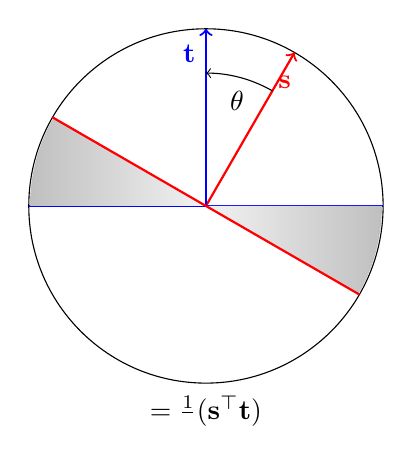
\begin{tikzpicture}[scale=1.5]

    % Circle
    \draw (0, 0) circle (1.5cm);

    % Vectors s (red at 60°) and t (blue at 90°)
    \draw[->,thick,red]  (0,0) -- (60:1.5cm) node[pos=0.7, above right] {\(\mathbf{s}\)};
    \draw[->,thick,blue] (0,0) -- (90:1.5cm) node[pos=0.75, above left] {\(\mathbf{t}\)};

    % Angle theta (between s & t)
    \draw[<-] (0,1.125) arc (90:60:1.125cm) node[pos=0.7, below left] {\(\theta\)};

    % Blue lines (perp. to t = 90°)
    \draw[thick,blue] (0,0) -- (-1.5,0);
    \draw[thick,blue] (0,0) -- ( 1.5,0);

    % Gray shading for overlap region
    \shade[left color=gray!50, right color=gray!10]
      (0,0) -- (-1.49,0) arc (180:150:1.5cm) -- cycle;
    \shade[left color=gray!10, right color=gray!50]
      (0,0) -- (1.49,0) arc (0:-30:1.5cm) -- cycle;

    % Red line(s) perp. to s (60°)
    \draw[thick,red]  (0,0) -- (150:1.5);
    \draw[thick,red]  (0,0) -- (330:1.5); % same as -30°

    % Overlap formula
    \node at (0,-1.75) {\( \AVGR = \frac{1}{\ND} (\mathbf{s}^\top \mathbf{t}) \)};

\end{tikzpicture}
\end{minipage}%
\hfill
%-------------------------------%
% Right image: 3D Overlap (conic sections + wedge)
%-------------------------------%
\begin{minipage}{0.48\linewidth}
\centering
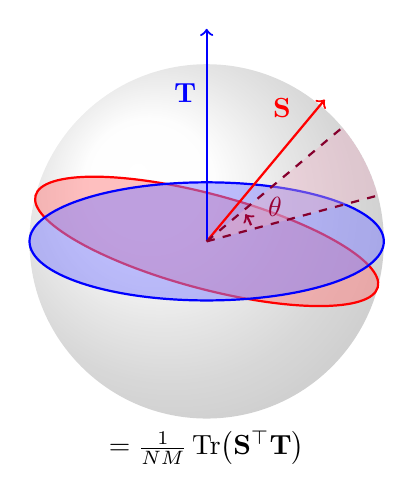
\begin{tikzpicture}[scale=1.5]

    % Light-gray "sphere"
    \shade[ball color=gray!5, opacity=0.3] (0,0) circle (1.5cm);

    % --- Red ellipse for S (unchanged) ---
    \begin{scope}
      \clip (0,0) circle (1.5cm);
      \fill[red!50, opacity=0.5]
        [rotate around={-15:(0,0)}, xscale=1.5, yscale=0.4]
        (0,0) circle (1.0);
    \end{scope}
    \draw[thick, red]
      [rotate around={-15:(0,0)}, xscale=1.5, yscale=0.4]
      (0,0) circle (1.0);

    % --- Blue ellipse for T (CHANGED) ---
    % Make it near-horizontal (rotate=0 or a small angle),
    % and bigger horizontally by increasing xscale significantly.
    \begin{scope}
      \clip (0,0) circle (1.5cm);
      \fill[blue!50, opacity=0.5]
        [rotate around={0:(0,0)},    % CHANGED: no tilt so near x-axis
         xscale=1.5, yscale=0.5]     % CHANGED: bigger horizontally
        (0,0) circle (1.0);
    \end{scope}
    \draw[thick, blue]
      [rotate around={0:(0,0)}, xscale=1.5, yscale=0.5]
      (0,0) circle (1.0);

    % Vectors S (red) & T (blue, vertical & longer)
    \draw[->,thick,red]  (0,0) -- (1.0,1.2)
      node[pos=0.8, above left]  {\(\mathbf{S}\)};
    \draw[->,thick,blue] (0,0) -- (0,1.8)
      node[pos=0.7, left] {\(\mathbf{T}\)};

    % Remove old "theta" arcs

    % -- Fill a wedge (solid angle) in purple --
    \begin{scope}
      \clip (0,0) circle (1.5cm);
      % Let’s pick a narrower wedge from ~15° to ~40°
      \fill[purple!30, opacity=0.4]
        (0,0)
         -- (15:1.5cm)
         arc [start angle=15, end angle=40, radius=1.5cm]
         -- cycle;
    \end{scope}

    % Dashed wedge boundaries
    \draw[thick, dashed, purple!70!black] (0,0) -- (15:1.5cm);
    \draw[thick, dashed, purple!70!black] (0,0) -- (40:1.5cm);

    % Single arc to label theta
    \draw[->, thick, purple!80!black]
      (20:0.4) arc[start angle=20, end angle=35, radius=0.4];
    \node[purple!80!black] at (27:0.65) {\(\theta\)};

    % Overlap formula
    \node at (0,-1.75) {\( \AVGR = \frac{1}{NM} \,\mathrm{Tr}\bigl(\mathbf{S}^\top \mathbf{T}\bigr) \)};

\end{tikzpicture}
\end{minipage}

% Main caption
\caption{Comparison of 2D and 3D representations of the vector and matrix Student--Teacher overlap \(R\).
\textbf{Left:} \(\AVGR = \tfrac{1}{\ND}\mathbf{s}^\top \mathbf{t}\).  Averaged over $\ND$ data samples (implicitly normalized to $1/m$).
\textbf{Right:} \(R = \tfrac{1}{NM}\,\mathrm{Tr}\bigl(\mathbf{S}^\top\mathbf{T}\bigr)\) with conic sections on the sphere (red \(\mathbf{S}\), blue \(\mathbf{T}\)), plus a purple wedge for the angle.  Averaged over matrix dimensions $N$ and $M$ (implicitly normalized over the data $1/\ND$).}
\label{fig:overlaps}
\end{figure}

%\caption{Comparison of 2D and 3D representations of matrix overlap $R$. (a) 2D visualization of vector overlap $R = \cos(\theta) $.
%  (b) 3D visualization of matrix overlap $R = \Trace{\frac{1}{N^2} \SMAT^\top \TMAT $ with solid angle $R$.}



%%\subsubsection{Derivation of the  ST error $(\EPSL(\AVGR))$ for the Linear Perceptron}
\paragraph{Derivation of the ST error $(\EPSL(\AVGR))$ for the Linear Perceptron.}
%\nred{WARNING: there may be some mistakes here}
To derive \EQN~\ref{eqn:LinearPerceptronError},
define the data-dependent ST error (\EQN~\ref{eqn:DE_L}) in terms of an $\ell_2$ loss function.

Write the data-averaged ST error as
\begin{align}
\nonumber
\DETOPSTLL= & \frac{1}{2} \sum_{\mu=1}^{\ND}(\Ys - \Yt)^{\top} (\Ys - \Yt)
\end{align}
Define the $\ND$ label vectors  
$\YsVEC:=[\YsIS{1}, \YsIS{2}, \cdots, \YsIS{\ND}]$ and 
$\YtVEC:=[\YtIS{1}, \YtIS{2}, \cdots, \YtIS{\ND}]$.
This lets us write 

\begin{align}
\nonumber
\DETOPSTLL= & \frac{1}{2} \Trace{(\YsVEC - \YtVEC)^{\top} (\YsVEC - \YtVEC)} \\
\nonumber
=& \frac{1}{2} \Trace{(\YsVEC)^{\top} \YsVEC - 2 (\YsVEC)^{\top} \YtVEC + (\YtVEC)^{\top} \YtVEC } \\
\nonumber
=& \ND - \Trace{(\YsVEC)^{\top} (\YtVEC)}\\
=& \ND- \Trace{\ETA(\SVEC,\TVEC,\red{\NDXI})},
\label{eqn:deriveSTerror}
\end{align}
where we define the \emph{data-dependent \SelfOverlap}:
\begin{equation}
\ETA(\SVEC,\TVEC,\red{\NDXI}):=(\YsVEC)^{\top}(\YtVEC)
\end{equation}

The expression $\ETA(\SVEC,\TVEC,\NDXI)$ is analogous to the ST overlap $R$, but before the data has been integrated out.
It is convenient to work directly with
the \SelfOverlap $\ETA(\SVEC,\TVEC,\NDXI)$ because it will appear later in \EQN~\ref{eqn:eta_mat_avg_def} (in Section~\ref{sxn:matgen}), 
when formulating the matrix-generalized overlap operator~$\OVERLAP$.

In defining $\ETA(\SVEC,\TVEC,\NDXI)$, we replace the individual labels $(\Ys,\Yt)$ with the Energy functions $E_{NN}$ that generate them, giving an expression in terms of the weights $(\SVEC,\TVEC)$ and the Gaussian data variables $(\XI)$. We will then integrate out the data variables, leaving an expression just in terms of the weights.  
Using the $E_{NN}$ Energy generating or output function (\EQN~\ref{eqn:dnn_energy}, \ref{eqn:S_ENN}, \ref{eqn:T_ENN}), we can write the labels as
\begin{align}
\Ys=\SVEC^{\top}\XI_{\mu},\;\;
\Yt=\TVEC^{\top}\XI_{\mu}  .
\end{align}
This now gives the data-dependent \SelfOverlap explicitly as
\begin{align}
  \label{eqn:eta_vec_xi_def}
\ETA(\SVEC,\TVEC,\NDXI) =\sum_{\mu=1}^{\ND} (\SVEC^{\top}\XI_{\mu})^{\top} (\TVEC^{\top}\XI_{\mu}) = \sum_{\mu=1}^{\ND}\XI^{\top}_{\red{\mu}}  (\SVEC^{\top} \TVEC )\XI_{\red{\mu}} 
\end{align}
After integrating over the data, we have the \emph{data-independent \SelfOverlap}, $ETA(\SVEC,\TVEC)$:
\begin{align}
\label{eqn:eta_vec_avg_def}
\ETA(\SVEC,\TVEC) := \langle\ETA(\SVEC,\TVEC,\NDXI)\rangle_{\AVGNDXI}
   = & \frac{1}{\ND}\int d\mu(\NDXI)\ETA(\SVEC,\TVEC,\NDXI) \\ \nonumber
= & \frac{1}{\ND}\int d\mu(\NDXI)\sum_{\mu=1}^{\ND}\XI_{\mu}^{\top}\SVEC^{\top}\TVEC\XI_{\mu} \\ \nonumber
= & \frac{1}{\ND}\int d\mu(\NDXI)\sum_{\mu=1}^{\ND}\XI_{\mu}^{\top}\AVGR\XI_{\mu} \\ \nonumber
= & \AVGR\;\frac{1}{\ND}\sum_{\mu=1}^{\ND}\int d\mu(\XI_{\mu})\XI_{\mu}^{\top}\XI_{\mu} \\ \nonumber
   = &\AVGR.
\end{align}

where the third equality holds because $\AVGR$ is a scalar constant, and the fourth holds because the elements of $\XI$ are i.i.d. and normalized to unit variance.
% Since $d\mu(\NDXI)$ is a measure over a (multi-variate) Gaussian distribution (i.e., $d\mu(\NDXI)=\mathcal{D}\NDXI P(\NDXI)$), and because data vectors $\XI$ are normalized you unity 
(See Section~\ref{app:st-gen-err-annealed-ham}) .

We can now obtain the \EffectivePotential $\EPSL(\AVGR)$ for the data-averaged ST test error (see \EQN~\ref{eqn:epsl}),  as in \EQN~\ref{eqn:LinearPerceptronError},
\begin{align}
\label{eqn:e0}
\EPSL(\AVGR)=\langle\DETOPSTLL\rangle_{\AVGNDXI} =  1 - \AVGR .
\end{align}

In traditional \STATMECH (e.g., \cite{SST92}), one is interested in how the \emph{\TotalModelGeneralizationError} $\TGE(\AVGR)$ depends on $\AVGR$.
With these simple error functions, \EQN~\ref{eqn:MGE} reduces to a function over $\AVGR$,
and the \AverageSTGeneralizationError $\STGE(\AVGR)$ is then obtained by averaging over the Students 
\begin{align}
\label{eqn:AVGSTGE_R}
\AVGSTGE(\AVGR)=\THRMAVG{\EPSL(\AVGR)}=
\THRMAVG{1-\langle\ETA(\SVEC,\TVEC,\NDXI)\rangle_{\AVGNDXI}}=
\THRMAVG{1-\ETA(\SVEC,\TVEC)}=
\THRMAVG{1-\SVEC^{\top}\TVEC}=
\THRMAVG{(1-\AVGR)}  ,
\end{align}
where $\THRMAVG{\cdots}$ is a \ThermalAverage over the \Student weight vector $\SVEC$.

The \ModelQuality for the ST \Perceptron, $\Q^{ST}$,
is just the \AverageGeneralizationAccuracy, so we can write
\begin{align}
\label{eqn:QST_final}
\Q^{ST} := 1 - \AVGSTGE(\AVGR) 
       = \THRMAVG{1 - \EPSL(\AVGR)} 
       = \THRMAVG{\langle\ETA(\SVEC, \TVEC, \NDXI)\rangle_{\AVGNDXI}} 
       = \THRMAVG{\ETA(\SVEC, \TVEC)} 
       = \THRMAVG{\SVEC^{\top}\TVEC} 
       = \THRMAVG{\AVGR}.
\end{align}
\EQN~\ref{eqn:QST_final} is the starting point for deriving a \SEMIEMP theory for the \WW quality metrics (\ALPHA,\ALPHAHAT);
see Section~\ref{sxn:matgen_mlp3}.
To generalize this expression, we will start with the \SelfOverlap $\ETA(\SMAT,\TMAT,\NDXI)$ for a
\MultiLayerPerceptron (MLP3) in Section~\ref{sxn:matgen}.

Before doing this, however, we note that we can obtain this expression for $\STGE$ by defining the
\AnnealedHamiltonian $\HANHT(\AVGR)$, at high-Temperature, as in Section~\ref{sxn:mathP}, \EQN~\ref{eqn:Gan_highT_final}.
Indeed, it is really $\HANHT(\AVGR)=\EPSL(\AVGR)$ that we must generalize to the matrix case, which we do (using a technique
similar to a Replica calculation, but still in the AA).
For more details, see Appendix~\ref{sxn:summary_sst92}.
(In particular, doing this allows us to define the normalization needed later for the \TRACELOG condition).
\michaeladdressed{MM TO DO: still to work on this par.}


\begin{table}[t]
  \raggedright
\hspace*{-1.5cm}% Adjust this value as needed
\renewcommand{\arraystretch}{1.25} % Increase line spacing in table
\begin{tabular}{|c|c|c|c|}
  \hline
  Quantity & Traditional \SMOG & \makecell{\LinearPerceptron \\ in Traditional \SMOG} & \makecell{Matrix Generalization \\ for \SETOL} \\ \hline

  Total (Idealized) Data Error 
    & $\DETOPXI$ (\ref{eqn:detox})
    & $\DETOPSTL$ (\ref{eqn:deriveSTerror}) 
    & $\DETOPNN$ (\ref{eqn:DE2}) \\ \hline

   Annealed Hamiltonian
    & $\HANHT=\EPSLw$ (\ref{eqn:epsl}) 
    & $\GANHTR=\EPSLSTx=1-\AVGR$ (\ref{eqn:epslR}) 
  & $\GANMATHT = N(\IM-\OVERLAP)$ (\ref{eqn:GANHTmatR}) \\

  (Data-Averaged Error) 
    & (AA, at high-T) 
    & (and at \LargeN) 
    & (only for a layer)  \\ \hline

    \SelfOverlap 
    & $\ETAw = 1-\EPSLw$~(\ref{eqn:def_eta})

    & $\ETA(\SVEC,\TVEC)=\SVEC^{\top}\TVEC$ (\ref{eqn:eta_vec_avg_def})
    & $\ETA(\SMAT,\TMAT)=\tfrac{1}{N}\SMAT^{\top}\TMAT$ (\ref{eqn:eta_mat_avg_def})  \\ \hline
    \hline

  \ModelQuality 
    & $\Q:=1-\AVGGE$ 
    & $\Q^{ST}:=1-\AVGGE^{ST}$ (\ref{eqn:model_qualities})
   & $\Q^{NN}:=1-\AVGGE^{NN}$  (\ref{eqn:model_qualities})\\ 

  in terms of \LayerQuality
    & 
    & 
   & $\Q^{NN}:=\prod_{L} \Q^{NN}_{L}$ \\ \hline
\end{tabular}
\caption{Summary of key quantities compared across traditional \SMOG models,  the \Student-\Teacher (ST) \LinearPerceptron--in the \AnnealedApproximation
(AA) and at high-Temperature (high-T) and at \LargeN in $\ND$, and the matrix-generalized forms as the starting point to frame \SETOL.
The total ST Error of Energy, $\DELBF$, represents the difference (squared) between the model and its labels for the ST model between
the \Student and \Teacher predictions.
The \AnnealedHamiltonian is the Energy function for this Error after it is averaged over the model for the training data
(an $\ND$-dimensional i.i.d. idealized Gaussian dataset,  $\NDXIn$).
In the AA, the \AnnealedHamiltonian is equal to the \EffectivePotential.  For the ST model,  this is one minus the average overlap, $\HANHT(R)=(1-\AVGR)$;
for the \SETOL, this is  the ($M$-dimensional) identity minus the overlap operator/matrix, $\HANHT(\OVERLAP)=N(\IM-\OVERLAP)$. 
The \SelfOverlap $\eta(\cdots)$ is used to describe the Accuracy (as opposed to the Error) for both the ST model and
its matrix-generalized form.
%Notice that $\eta(\XI)$, as defined,  has not yet been averaged over the model data $\XI^{N}$.
Finally, the different forms of the \Quality are defined.  Generally speaking, the \Quality $\Q$ is an approximation to some measure
of $1$ minus the \AverageGeneralizationError, $\Q:=1-\AVGGE$ (in the AA, at high-T, at \LargeN, and with whatever else
approximations are applied).
For the ST model, having just 1 layer, the \ModelQuality and the \LayerQuality are the same, and denoted $\Q^{ST}$.
For \SETOL, the \ModelQuality $\Q^{NN}$ is a product of individual \LayerQualities $\Q^{NN}_{L}$.
(Note that the  final \SETOL \LayerQuality $\Q$ is defined in terms of the \LayerQualitySquared $\QT$,
and the starting point for this is expressed with the \LayerQualitySquared Hamiltonian $\HBARE=\OLAPTOLAP$.
}
\label{table:quantities_general_vect_matrix}
\end{table}

